 %!TEX TS-program = xelatex
%!TEX encoding = UTF-8 Unicode

%\def \papersize {a5paper}
\def \papersize {a4paper}
%\def \papersize {letterpaper}

%\documentclass[14pt,\papersize]{extarticle}
\documentclass[12pt,\papersize]{extarticle}
% extarticle is like article but can handle 8pt, 9pt, 10pt, 11pt, 12pt, 14pt, 17pt, and 20pt text

\def \ititle {Origins of Mind: Lecture Notes}
\def \isubtitle {Lecture 01}
%comment some of the following out depending on whether anonymous
\def \iauthor {Stephen A.\ Butterfill}
\def \iemail{s.butterfill@warwick.ac.uk% \& corrado.sinigaglia@unimi.it
}
%\def \iauthor {}
%\def \iemail{}
%\date{}

%\input{$HOME/Documents/submissions/preamble_steve_paper4}
\input{$HOME/Documents/submissions/preamble_steve_lecture_notes}

%no indent, space between paragraphs
\usepackage{parskip}

%comment these out if not anonymous:
%\author{}
%\date{}

%for e reader version: small margins
% (remove all for paper!)
%\geometry{headsep=2em} %keep running header away from text
%\geometry{footskip=1.5cm} %keep page numbers away from text
%\geometry{top=1cm} %increase to 3.5 if use header
%\geometry{bottom=2cm} %increase to 3.5 if use header
%\geometry{left=1cm} %increase to 3.5 if use header
%\geometry{right=1cm} %increase to 3.5 if use header

% disables chapter, section and subsection numbering
\setcounter{secnumdepth}{-1}

%avoid overhang
\tolerance=5000

%\setromanfont[Mapping=tex-text]{Sabon LT Std}


%for putting citations into main text (for reading):
% use bibentry command
% nb this doesn’t work with mynewapa style; use apalike for \bibliographystyle
% nb2: use \nobibliography to introduce the readings
\usepackage{bibentry}

%screws up word count for some reason:
%\bibliographystyle{$HOME/Documents/submissions/mynewapa}
\bibliographystyle{apalike}


\begin{document}



\setlength\footnotesep{1em}






%---------------
%--- start paste

\title {Origins of Mind \\ Lecture 05: Knowledge of Colour}



\maketitle

\subsection{slide-3}
Recall from the previous lecture that our Next Big Problem is this.
We've said that infants' competence with causes and objects is not knowledge but something
more primitive than knowledge, something which exists in adults too and can carry information
discrepant with what they know. So, if at all, how does appealing to these early capacities
enable us to explain the origins of knowledge?

Versions of this problem will arise in every domain of knowledge we shall consider.
In this lecture I want to consider our Next Big Problem by thinking about the domain of colour.
We are also, of course, simultaneously occupied with a question about the origins of knowledge
of colour.
Let me start by introducing the question ...

--------
\subsection{slide-4}
Diagram: years bewteen early capacities (core knowlegde) and knowledge proper



\section{Knowledge of Colour: a Question}

\subsection{slide-5}
Let me start with something quite basic.
Here are three patches of colour.
The patches are all different colours, but the two leftmost are both the same colour---they are both blue.
This sounds contradictory but isn't.
In one case we're talking about the particular colours of things; in the other case we're talking about colour category.

The question I want to ask about knowledge of colour concerns these cateories.
You know that these two are both blue whereas this is not (it's green).
How do you come to know this?
(Ask them to discuss.)
Does anyone thing the answer is that you can just see it?  As we'll see, that idea looks promising initiall but it's not quite that simple.

*TODO*: \citep{webster:2012_color} has good summary and lots of complications about CP.
Also introduces methods not considered here.

\subsection{unit\_111}


\section{Categorical Perception of Colour}

\subsection{slide-8}
Remember the idea that words like 'blue' pick out colour categories?

To claim that there is categorical perception is, very roughly and to a first approximation, to claim that perceptual processes are concerned not only with the particular colours of things but also with categories of colour like blue and red.

This is not a definition, only a very rough starting point.

\subsection{slide-10}
I can't tell you what categorical perception is.
The operational definitions used in psychology are unrevealling.
And the ways philosophers define it are wrong, or at least depend on unjustified
assumptions.

\subsection{slide-12}
But how can we study it without knowing what it is?
We have to proceed by seeing what conclusions about it are supported by evidence.
Then we can work back to infer what it is by asking what it could be if these
conclusions are true.
Put differently, we can start by asking, What is categorical perception commonly
taken to explain?

\subsection{slide-13}
At this point we should take nothing for granted and make no assumptions about what
sense, if any, categorical perception involves either categories or perception.
We  are only asking, What is categorical perception commonly taken to explain?

\subsection{slide-14}
What is categorical perception of colour commonly taken to explain?
The diagram below represents sequences of three colours.
The vertical sequence shows three greens and the uppermost horizontal sequence shows a
blue, a purple and a pink.
div \begin{center}
div 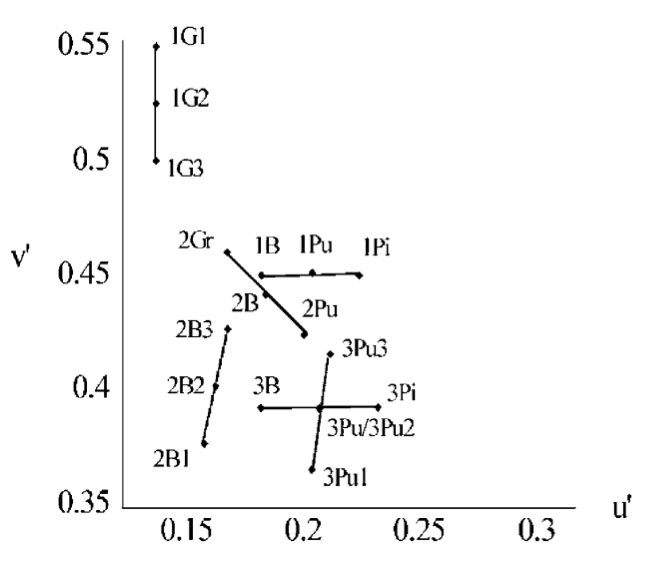
\includegraphics[scale=0.3]{daoutis_2006_fig_A1.png}
div \end{center}
div \begin{center} \citealp{Daoutis:2006ij} figure A1 \end{center}

\subsection{slide-15}
Each colour differs from its neighbours by the same amount according to a standard
measure based on the human eye's abilities to discriminate wavelengths.

\subsection{slide-16}
Yet the greens are often judged to look quite similar and the blue-pink-purple to look very different \citep[p.\ 12--7]{Roberson:1999rk}.
When people are asked to name these colours, they often give the same name to the greens but different names to members of the blue-pink-purple sequence.
And people are generally faster and more accurate in discriminating between members of the blue-pink-purple sequence than members of the green sequence
(faster: \citealp{Bornstein:1984cb}; more accurate: \citealp[p.\ 22--7]{Roberson:1999rk}).

Yet the greens are often judged to look quite similar and the blue-pink-purple to look very different \citep[p.\ 12--7]{Roberson:1999rk}.
When people are asked to name these colours, they often give the same name to the greens but different names to members of the blue-pink-purple sequence.
And people are generally faster and more accurate in discriminating between members of the blue-pink-purple sequence than members of the green sequence
(faster: \citealp{Bornstein:1984cb}; more accurate: \citealp[p.\ 22--7]{Roberson:1999rk}).

\subsection{slide-17}
Let me show you how speed an accuracy of discimination are usually measured.

This is a 2-alternative forced-choice task (2AFC).

\subsection{slide-20}
So far we've talked about three ways in which the blue-pink-purple sequence differs
from the greens.
The green sequence also differs from the blue-pink-purple sequence on other measures.

\subsection{slide-21}
But these results are not confined to just two sequences.
There is a way of dividing a colour space into categories that predicts all of these
results and more.
When the members of a sequence of colours fall into different categories, the colours
are said to look very different, they are given different verbal labels, and the
subject can discriminate them faster and more accurately than when they don't fall
into different categories (all other things being equal).
The fact that, for an individual subject, all these effects are predicted by a single
way of dividing the colour space into categories is what categorical perception of
colour is supposed to explain.

\subsection{categorical\_perception\_df}
Now we're in a position to say what categorical perception is.
A single way of dividing up the colour similarity space into a small finite number of
equivalence classes enables us to predict a variety of effects including patterns in:
reports of phenomenal similarity and difference, the use of linguistic labels, and
speed and accuracy of discrimination.

\subsection{slide-24}
This is a fact in need of explanation.

\subsection{slide-27}
So what is categorical perception?
Categorical perception is the process, whatever it is, that explains the unexpected effects.
Now this way of defining categorical perception is not very informative.
This is a virtue---categorical perception is something to be discovered, not defined.
We might ask, what sort of process is categorical perception?
In particular, we might wonder whether and in what sense it is a perceptual process.
How can we discover more about categorical perception?
One way to do this is to look for further unexpected patterns to be explained.
It's just here that pop-out is useful.

\subsection{slide-28}
Another measure on which the green sequence differs from the blue-pink-purple sequence is pop-out, which is defined operationally in terms of visual search tasks \citep[p.\ 117]{Treisman:1986pm}.
First I need to explain what a visual search task is.
In visual search tasks tasks, subjects are shown an array of objects and asked to identify the one with a certain property.
For example, one might be shown an array of twenty animal pictures and asked to identify the cat.
Normally the time it takes subjects to find a target increases linearly as the number of objects in the array increases.
But when the target of a visual search is defined in terms of colour and the colours of the distractors are categorically different from the colour of the target, subjects can find the target just as quickly when it is in among 36 distractors as when there are only four distractors \citep[Experiment 1]{Daoutis:2006qk}.
This is, the colours pop out.

\subsection{slide-35}
Recall that we defined categorical perception in terms of things it could explain.
Now we can add pop-out to that list.
This gives us more insight into what categorical perception is.
In particular, it indicates that categorical perception is a perceptual process.
And we can go on finding out more about categorical perception by finding out more about the things it explains.
This is why I refused to define it at the start, and why you have to start without knowing what categorical perception is.

\subsection{slide-36}
Our topic is still categorical perception, but I want to pause here to reflect on how
we've defined categorical perception.
We should think of core knowledge using the same method.
At the outset we don't know what core knowledge is.
I just said it's like knowledge in some ways but not knowledge.
We'll get a handle on it by looking at what it is commonly supposed to explain.
More on this later; now back to categorical perception.

\subsection{slide-38}
Among the things categorical perception is commonly taken to explain there are also automatic processes.

(This will be important later.)

\subsection{slide-39}
For an example of a category effect which is automatic, I need to introduce you to the odd-ball paradigm.

In the odd-ball paradigm, you see a series of things that are all the same; and then, unpredictably, you see something different.

We can use sensitivity to odd-balls to measure the difference between the two blues and the blue-green pair.

This is useful because odd-ball effects can be detected very early in visual processessing, before attention kicks in.

They allow us to probe automatic processes.

\subsection{slide-49}
Now suppose we play you an odd ball sequence.
We want to know whether an automatic process picks up on the difference.
And we want to know whether the automatic process picks up on the difference always or only when a category change is involved.
To do this we need to measure an event-related potential called vMMN (which is short for visual mismatch negativity).

\subsection{slide-50}
Now I need to explain what an event-related potential is.

\subsection{slide-53}
An ERP like the vMMN stands to an overall EEG measurement a bit like the number 78 bus does to a collection of atoms.

\subsection{slide-54}
While we're on methods, let's quickly talk about fMRI.

\subsection{slide-57}
So now we know what an event-related potential is, let's get back to the vMMN (visual mismatch negativity).

\subsection{slide-58}
So let me show you a task that uses this odd-ball effect
Fixate on this cross.
And when you see the rectangle, press the space bar with both index fingers.
That's it.
Except that you also see a block of colour on every trial.
You're instructed to ignore this block of colour.
And generally that's easy because it's always the same colour.
But just occasionally it's a different colour.
In one condition, the usual and odd-ball colours are the blues.
And in the other condition, the usual and odd-ball colours are cross-category, from blue-green.
We're interested in whether there's a sign that your brain has detected the change when the odd ball colour occurs.

Put roughly, the results show that there is signal of pre-attentive change detection at around 100-200 milliseconds in the left visual field.

\subsection{slide-63}
This is another way of presenting the same finding.

The vMMN is a DRN, but not all DRNs are vMMNs (see the paper).

\subsection{slide-65}
Recall that we defined categorical perception in terms of things it could explain.
Now we can add a further item to that list: odd-ball detection.
Again, this gives us more insight into what categorical perception is.
In particular, it indicates that categorical perception is an automatic process.
It isn't only a matter of how you experience things to be.

\subsection{unit\_121}


\section{Categorical Perception in Infancy}

\subsection{slide-67}
Categorical perception of colour emerges early in infancy, from around four months or earlier, as has been demonstrated using habituation (Bornstein, Kessen
and Weiskopf 1976).

\subsection{slide-72}
Categorical perception has also been demonstrated at four months of age using pop-out (Franklin, Pilling and Davies 2005).

\subsection{slide-78}
Slightly older infants can also make use of colour properties such as red and green to recognise objects.  For instance, nine-months-olds can determine whether an object they saw earlier is the same as a subsequently presented object on the basis of its colour (Wilcox, Woods and Chapa 2008).

\subsection{slide-79}
By the time they are two years old, toddlers who do not comprehend any colour terms can use colour categories implicitly in learning and using proper names; for instance, they are able to learn and use proper names for toy dinosaurs that differ only in colour (Soja 1994: Experiment 3).

So we see categorical perception of colour early in development and it is useful to children.

\subsection{slide-80}
Infants enjoy categorical perception not only of colour but also of orientation (Franklin et al. 2010), speech (Kuhl 1987, 2004; Jusczyk 1995) and facial
expressions of emotion (Etcoff \& Magee 1992; Kotsoni et al. 2001; Campanella et al. 2002).

\subsection{slide-96}
To recap, infants enjoy categorical perception not only of colour but also of orientation (Franklin et al. 2010), speech (Kuhl 1987, 2004; Jusczyk 1995) and
facial expressions of emotion (Etcoff \& Magee 1992; Kotsoni et al. 2001; Campanella et al. 2002).

\subsection{unit\_131}


\section{Categorical Perception and Knowledge}

\subsection{slide-99}
Recall that our Next Big Problem is this.
We've said that infants' competence with causes and objects is not knowledge but something
more primitive than knowledge, something which exists in adults too and can carry information
discrepant with what they know. So, if at all, how does appealing to these early capacities
enable us to explain the origins of knowledge?

As we've just seen, a version of this problem arises for the case of colour.
Perhaps we can partially resolve the Next Big Problem in the case of colour, and then use
this as a model for other cases.

Let's see.
First I want to be clear about what the problem is ...

\subsection{slide-100}
Our overall question is about how humans come to know things about colours.

How is categorical perception of colour relevant to this question?

\subsection{slide-101}
Harnad offers a hypothesis which might seem natural to accept at this point.

\subsection{slide-102}
Incidentally, Spelke also uses the building blocks metaphor.

But of course Spelke is talking about core knowledge rather than categorical perception.  (I think the two might be related, but I suspect she would strongly disagree.)

\subsection{slide-104}
But is it true?

\subsection{slide-105}
The first problem is to understand the ‘building blocks’ metaphor.

\subsection{slide-108}
We'll say something about what modules are later---for now, just be aware that categorical perception counts as a modular process.

\subsection{slide-109}
Here's a first attempt to understand the ‘building blocks’ metaphor.
Let's suppose that categorical perception of colour amounts to having colour concepts.
This way of thinking concords with Leslie's view about modular cognition.

\subsection{slide-111}
The toy is put away so that the subjects couldn't see it.

\subsection{slide-110}
It can't be right that having categorical perception of colour (or X) amounts to having colour (or X) concepts.
We know this can't be right because there is a gap of two or more years between categorical perception of colour and possession of colour concepts.
For consider what is involved in having a colour concept.
It is not just responding differently to red things than to green things (say).
It also requires

\subsection{slide-116}
Kowalski and Zimiles' paradigm provides an excellent operationalisation of concept possession.

We should hold in mind the idea that having a concept of something involves being able to think abstractly about that thing.

\subsection{slide-117}
But for now Kowalski and Zimiles are important because they show that having categorical perception of colour is not the same thing as having colour concepts.

\subsection{slide-118}
So the first view can't be right.
It can't be right that having categorical perception of colour (or X) amounts to having colour (or X) concepts.
And the same applies in other cases of categorical perception as well.
(Of course a defender of the view that categorical perception is or entails concept possession might insist that subjects have concepts but cannot use them,
at least not in the sort of task I have just described. This is possible, of course, but it seems to be a desperate defence.)
How else might we understand the ‘building blocks’ metaphor?

\subsection{slide-120}
One worry here is that we've replaced one metaphor with another, ‘redescription’ for ‘building block’.
But let's put this aside for a moment in order to reflect on why Mandler is wrong.

\subsection{slide-121}
Consider Mandler's claim that
‘the earliest conceptual functioning consists of a redescription of perceptual structure’ (Mandler 1992)

\subsection{slide-122}
The boundaries of adults' perceptual categories do not match the boundaries of infant and toddler perceptual categories.
How do we know?
First note that the extensions of colour terms vary between languages.

\subsection{slide-123}
Indeed, the extensions of colour terms vary quite radically between languages.
Ongoing research concerns whether there is any kind of universal prinicple behind the pattern.

\subsection{slide-125}
So the extensions of colour terms varies between langauges.

Why is this relevant to the relation between infant and adult categorical perception?

\subsection{slide-126}
Because the boundaries of adults' (but not infants') perceptual categories are
influenced by the extensions of their culturally variable colour terms.

For evidence that adults' perceptual colour categories are influenced by their
culturally variable knowledge of colour words, see \citet{Kay:2006ly},
\citet{Roberson:2007wg}, and \citet{Winawer:2007im};

This is an amazing finding about the power of words.

Learning to use words for colours changes how we perceive them.

Colour words shape adults’ categorical perception \citep{Roberson:2007wg,Winawer:2007im}.

We'll see more on this later.

\subsection{slide-127}
But, as you'd expect, infants’ and toddlers’ perceptual categories are not influenced by the extensions of colour terms.

For evidence that toddlers who know some colour words show no influence of language on categorical perception of colours, see \citet{Franklin:2005hp}.

\subsection{slide-129}
So the second view probably isn't right either.
For whatever redescription amounts to, it should surely involve there being some kind of match between the perceptual categories and the concepts.
And, on the face of, it there is no match at all.

\subsection{slide-130}
So what are we to make of the ‘building blocks’ idea?
It may be that we have to reject the building blocks idea altogether.
For infant categorical perception of colour seems only very distantly related to adult uses of colour concepts.
Does this mean that categorical perception plays no role at all in explaining the emergence of knowledge about colours?
No, we haven't shown that.  Only that categorical perception alone is not enough; and also that
it is hard to understand exactly how categorical perception plays a role in the emergence of knowledge.

\subsection{slide-132}
The role of some early-developing abilities in explaining the later acquisition of conceptual
understanding does not involve direct representational connections; rather the early developing
abilities influence attention and inform behaviour, and these influences facilitate
development.

\subsection{slide-133}
What is missing from the building blocks idea is adequate recognition that social interaction is
important for the emergence of knowledge.

Here is a bold conjecture about how humans come to know things.

\subsection{slide-134}
The challenge, of course, is to say *how* social interaction enables humans to come to know
things.

\subsection{slide-135}
In emphasising rediscovery I want to identify a major role for social interaction while
also recognising the importance of the early developing representations of colours, objects
and causes.

The idea is, roughly, that coming to have knowledge involves rediscovering information that is
already represented.

\subsection{slide-136}
How might the idea of development as rediscovery apply in the case of knowledge of colour?

In acquiring a colour concept or word you need to:

\subsection{slide-137}
On locating the boundaries, I think having colour words might be helpful as a way of
marking a category before you know where its boundaries are.
That is, the word allows you to re-identify a category without knowing where it begins
or ends.

Given differences between the boundaries of pre-verbal infants' perceptual categories
and the extensions of colour words, it seems unlikely that categorical perception could
help here.  (Although it is possible in principle that, due to abstract features common to
all languages' systems of colour words, categorical perception might help; see Kay and ?*.)

\subsection{slide-138}
It's with this first problem that I think categorical perception helps with.
I suggest that categorical perception enables you to lock onto the relevant dimension.

How?
Categorical perception alters your experience so that there's a correspondence between
(i) changes on the relevant dimension, and (ii) changes in one phenomenal aspect of your
experience.
This correspondence helps you, eventually, to lock onto the relevant dimension and so to
acquire concepts and words.
Let me illustrate.

\subsection{slide-139}
One effect of categorical perception is phenomenological.
Consider the (a) difference between an experience of the first blue and the second blue;
and (b) the difference between an experience of the second blue and the green.
Phenomenally, the second pair of experiences is more different than the first.
There is some kind of phenomenological marker of categorical colour properties.
To put it colourfully, there is something that it is like for you to experience blue, and something else that it is like for you to experience green.
So, to return to the two problems, this is why I think categorical perception might be important for identifying the dimension.

\subsection{slide-140}
Let me return to the picture I finished with at the end of the last lecture.

This picture is about core knowledge, but I think we should broaden that to include categorical perception.
In fact I think core knowledge and categorical perception are likely to be closely related, as I'll explain later.

The question for this lecture was, how do we come to know things about colour.
The answer, I think, is this.
We have categorical perception of colour from early in infancy, certainly from around four months of age.
Having categorical perception is not by itself sufficient for having colour concepts.
But it does play an important role, because it means that there is
a correspondence between (i) changes on the relevant dimension, and (ii) changes in one phenomenal aspect of our experience.
I conjecture that this helps us to identify the relevant dimension, colour not shape or size, in acquiring colour words and concepts.
But by itself this is not enough.
As we've seen, acquiring colour concepts also depends on having some colour words.
I speculate that this is because words function as a tool for marking categories prior to knowing where they start and end.
The word allows you to re-identify a category without knowing where it begins or ends.

So this is my picture.
Acquiring knowledge of colour depends on an interaction between categorical perception, something developmentally quite primitive, and social interaction, in
particular the negotiation of words for colour categories.

\subsection{slide-141}
To conclude, we've seen that although infants enjoy categorical perception of colour from four months or earlier,
this doesn't straightforwardly explain how they come to know about the colours of things.
In particular, having categorical perception does not entail having a concept.
Nor does having a concept seem to be a matter of somehow redescribing or latching on to what is catgeorically perceived.
On the other hand, having colour words and being able to use them accurately does seeem to matter for the acquisition of knowledge of colour.
So this is one example where having verbal labels for things may help with acquiring concepts of them.

\subsection{unit\_141}


\section{Appendix: Categorical Perception in Infants and Adults (Optional)}

\subsection{slide-145}
Earlier I mentioned that infant and adult categorical perception of colour involve different colour categories.
Adults’ perceptual colour categories are shaped by their knowledge of words, whereas infants’ are not.
This means we should ask, What is the relation between infant and adult categorical perception?
A natural hypothesis is that they are one and the same, so that the infant categories transform into the adult ones.
This natural hypothesis turns out to be wrong.
Before explaining why, let me introduce one more puzzling finding.

\subsection{slide-147}
Let me show you how this works (roughly following Wiggett and Davies 2008)

Recall from earlier how speed and accuracy were tested using a two-alternative forced-choice task.

\subsection{slide-151}
Now Wiggett and Davies 2008 adapted this very slightly.

They put a word on the target (or, in Experiment 2, on the test stimuli --- that had no effect, showing that the word is important for priming and categorical perception is not a matter of matching label to label).

(They are using the Stroop effect, which I won't explain here but is worth looking up.)

\subsection{slide-153}
And here are the results from Experiment 1B.  The vertical axis is mean accuracy.

\subsection{slide-155}
Why say that impact of verbal interference plus shaping of perceptual categories by extensions of words gives an interesting sense in which we have expeirences as of red because we label perceived objects 'red'?  Two points: long-term, the extentions of perceptual category is influenced by the extension of the word; short-term, covert labelling primes the perceptual category and without this priming you do not have CP (Wiggett and Davies 2008).

\subsection{slide-156}
These findings leave us with a puzzle.
In adults, categorical perception of colour depends on the availability of linguistic labels for colour.
But infants lack such labels yet still manifest categorical perception.
How is this possible?
I think we have to resolve the puzzle by recognising that infant and adult categorical perception are different processes.

\subsection{slide-157}
The adult mode of categorical perception of colour differs from the infant-and-toddler mode in at least four respects: it disappears in the face of
predictable verbal interference but not non-verbal interference (Roberson, Davies and Davidoff 2000: 985; Pilling, Wiggett, et al. 2003: 549-50; Wiggett and
Davies 2008), it can be affected by short-term perceptual learning (Ozgen and Davies 2002), it depends on parts of the brain other than those on which
infants' categorical perception of colour depends (Franklin, Drivonikou, et al. 2008), and the boundaries of adults' perceptual categories do not match the
boundaries of infant and toddler perceptual categories.

\subsection{slide-158}
There is evidence that the infant mode of categorical perception of colour continues to operate in adults, although it is often inhibited or overshadowed
by the adult mode \citep{Gilbert:2006yb}.

\subsection{slide-159}
Our question was how humans make the transition from not being in a position to know that these are blue but this is not to being in a position to know this.
The appearance of categorical perception of colour at around four months of age made attractive the idea that the knowledge might come from, or be based on,
perception.
The tempting thought was that categorical perception of colour somehow provides a building block for colour concepts.
We saw that there were some reasons, not conclusive but quite powerful, to reject this idea.
In its place I offered a conjecture about development as rediscovery.
That conjecture was that in thought we rediscover something that our brains are already able to process, namely colour categories.
This suggests a certain amount of duplication. There's both a low-level cognitive process and a conceptual processes that deal with colour, that are not
directly linked by representations but rather only indirectly, via experience, the body and behaviour.
What we've just seen is that there is even more duplication than this suggests.
There are not just one but two perceptual processes which are concerned with categorising colour.
These appear to operate largely independently of each other, to have different neural bases and to be quite different kinds of process.
Minds are more complex than you think.

%--- end paste
%---------------






\bibliography{$HOME/endnote/phd_biblio}



\end{document}
